
\section{Testing}

For most duration of the project, testing was blackbox and manual. Tests were conducted for synchronization of various file names (characters) and formats. This brought out bugs in json formatting, file name encoding and HTTP request format.\newline

Furthermore, we also learned and configured test environment of Mocha, Chai and Sinon for the desktop application. We tried to implement the jsunit test. Due to lack of time to research more, it could not be completed.\newline

Some of the specific issues found on the desktop client, include:\newline
\begin{itemize}
\item{PDF file with characters such as space,-,'' can be downloaded but cannot be opened. Other PDFs can.}\newline
\item{File name with ' can be deleted in the local folder but cannot be deleted by using the delete button which invokes server delete.}\newline
\item{File with special symbol(*\&) can be uploaded but cannot be downloaded.}\newline
\item{In addition to non-standard named symbols, file names with special symbols (non-ASCII) cannot be renamed, but a new file with those symbols in their name can be uploaded.}\newline
\item{Batch delete/upload does not work.}\newline
\end{itemize}

The test case results are as shown below for Desktop client:\newline

\begin{figure}[H]
\centering
\subfigure[Upload,Download,Delete]{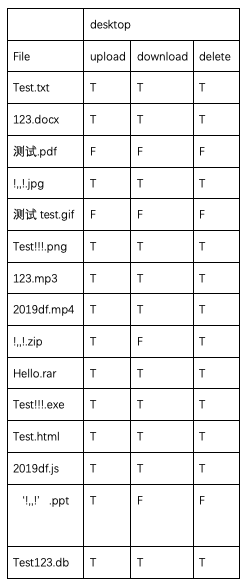
\includegraphics[width=60mm]{UDD.png}}%
\subfigure[Edit and Rename]{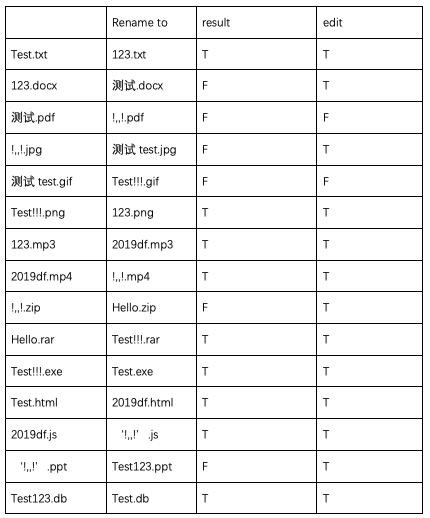
\includegraphics[width=60mm]{Rename.png}}
\end{figure}

The test case results for Mobile Client are as shown. Adding files are not as simple on Mobile as it is on Desktop and thus, the test cases are different:\newline

\begin{figure}[H]
\centering
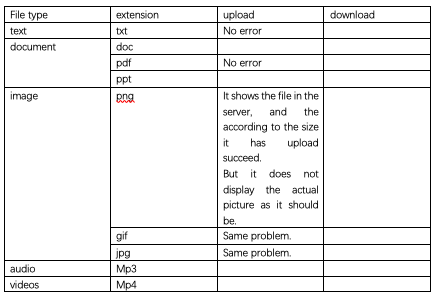
\includegraphics[scale=0.5]{mobiletest}
\end{figure}

\newline